

\subsection{Alkuperäinen ominaisuus ja parannus kohteet}

%toinen kappale pitää muokata

% ominaisuuden yhteenveto pitää lisätä tekstiä ellei se siirretä kokonaan koko yhteenvetoon



Sovelluksen "Progressio"{} sivulla on ominaisuus, 
joka antaa mahdollisuuden käyttäjälle seurata ja tallettaa hänelle annettua "mitattavaa"{} arvoa.
Kuvassa \nextImageCount {} näkyy on progressio sivu, 
ja siitä Käyttäjä pystyy valitsemaan miltä päivältä arvo on otettu ja mikä itse arvo on.
\medskip

\bigskip
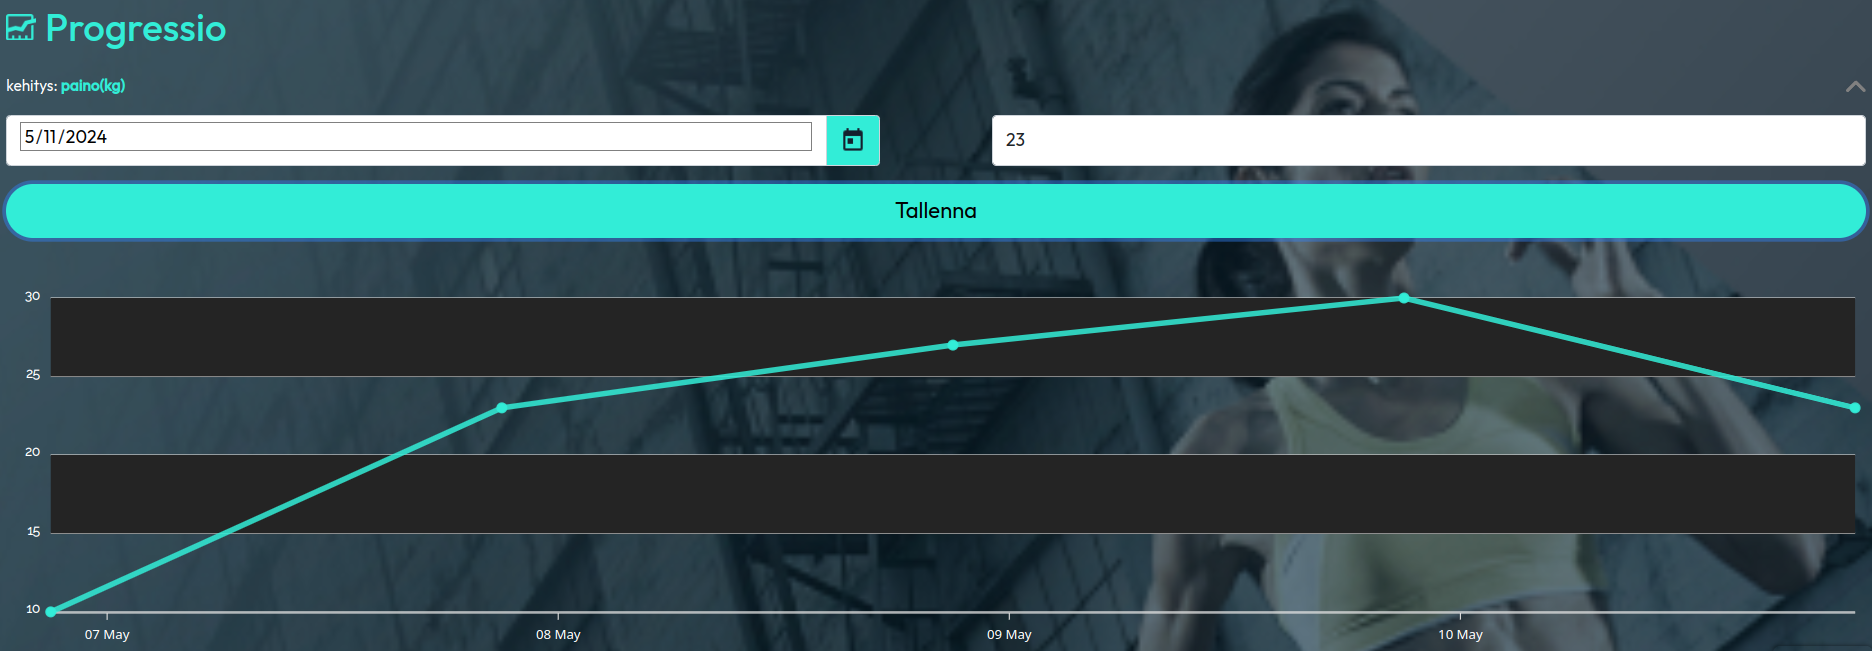
\includegraphics[width =15cm]{src/public/progressiosingle.png}\\
Kuva \getImgCount {}. Progressio sivu (tarvitsee paremman kuvan)
\medskip


% pitää muokata sanoitusta että se olisi järkevä

Kuvassa \theimgCounter {} mitattavan arvon suure on paino. 
% 
Tällä hetkellä käyttäjälle voi määrittää vain yhden mitattavan arvon, jota seurata.
Sain tehtäväksi laajentaa ominaisuutta siten että käyttäjälle voi määrittää useamman mitattavan arvon.
\medskip


Käyttäjän mitattavan arvon suure säilytetään käyttäjän profiilissa merkkijonona. 
Yksittäinen "measurableThing"{} ominaisuus ei ole riittävä useamman mitattavan arvon seurantaan, joten se pitäisi vaihtaa.
%
%mainitse paremmin mongo nosql dokumentti
% elä aloita koska sanalla
%Koska käytössä on NoSql dokumentti, voimme vaihtaa 
NoSql dokumentti tietokannan avusta "measurableThing"{} merkkijonon voi vaihtaa, "measurableThings"{} merkkijono listaan.
% voi vaihtaa merkkijono listaan ilman että pitää päivittää tietokanta pohjaa
% voidaan vaihtaa huoletta
% voidaan vaihtaa helposti
\medskip






\subsection{Ominaisuuden totetus}


\subsubsection{Käyttäjä profiili skeeman migraatio}



Käyttäjän mitattavan arvon vaihtaminen listaan vaatii käyttäjän skeeman muutoksen.
MongoDB:n NoSql dokumentti ei määritä tiukkaa skeemaa, joten käyttäjien skeemat voivat olla eriävät.
Skeeman muutos vaatii jokaisen käyttäjän profiilin muokkaamista haluttuun muotoon.
Käyttäjä profiilin skeeman muutos pitää tehdä kaikille aktiivisille käyttäjille, käyttäjän luontia pitää myös muokata siten, 
että uudet käyttäjän alkaisivat käyttämään uutta skeemaa.
\medskip

MongoDB antaa tallettaa mitä tahansa sen tietokantaan, joten projektissa on omat tyyppitarkastukset MongoDB rajapinnoissa, 
ettei virheelliset kirjoitus ohjeet talleta mitään tietokantaa.
%api muutos 
Nämä rajapinta tyyppitarkastukset pitää myös muokata sopimaan uuteen skeemaan.
\medskip

Migraatio tehdään kuvan \nextImageCount {} migraatio funktiolla. 
Funktio käy läpi kaikki käyttäjät, jolla on olemassa measurableThing ominaisuus ja päivittää sen measurableThings listaan.
Projektissa on tarpeeksi vähän käyttäjiä, joten migraatio tehdään synkronisesti palvelimella. 
Jos projektissa olisi isompi määrä käyttäjiä tämä operaatio pysäyttäisi palvelimen migraation ajaksi, kun käyttäjä profiileja päivitettäisiin.
Isoimmilla käyttäjä määrillä tämä operaatio tehtäisiin huolto aikana, jolloin sovellus ei olisi käytössä tai asynkronisesti, 
jolloin migraatio tapahtuisi pikkuhiljaa. 
\medskip

\bigskip
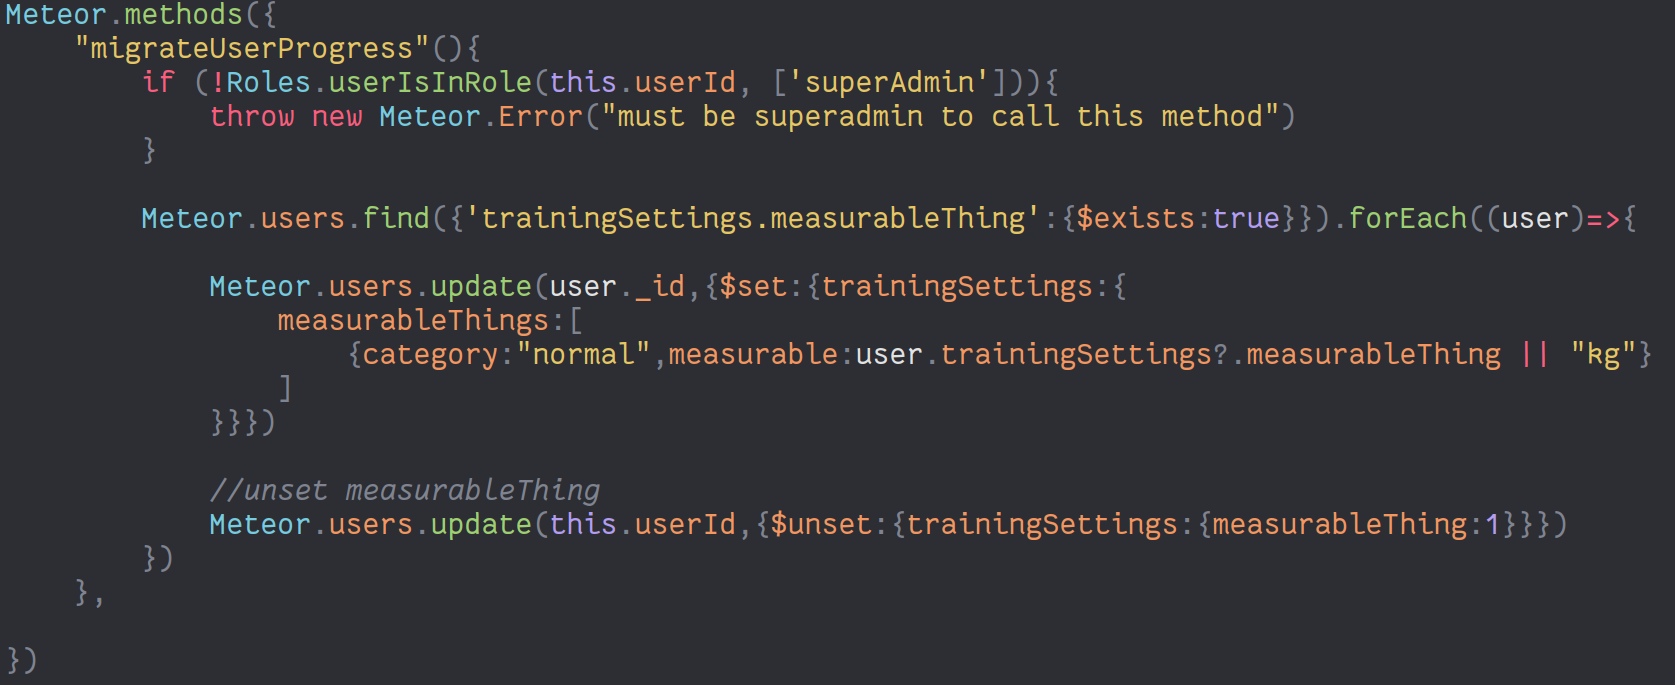
\includegraphics[width =15cm]{src/public/oppar/migrationfunction.png}\\
Kuva \getImgCount{}. Migraatio funktio
\medskip







\subsubsection{Käyttöliittymä}

%kappaleisiin voisi lisätä pari lausetta lisää




Käyttöliittymiä pitää muokata tukemaan ominaisuutta.
Käyttäjän luonti ja päivitys sivua pitää muokata siten, että käyttäjille voidaan antaa useita mitattavia arvoja.
Käyttäjän käyttöliittymää pitää muokata siten,
että käyttäjä voi vaihtaa mitä mitattavaa arvoa hän haluaa seurata tai mihin mitattavaan arvoon hän haluaa tallentaa lukemia.
%more
\medskip

Kuvassa \nextImageCount{} on käyttäjäpuolen käyttöliittymä muutoksien jälkeen.
Käyttöliittymässä käyttäjällä on mahdollisuus valita mihin mitattavaan suureeseen hän haluaa tallettaa arvoja kuvan {\the\numexpr \theimgCounter + 2 } laskuvalikolla.
% more words or fix something
Sivun kaavioon on myös lisätty mahdollisuus seurata monta mitattavaa arvoa.
\medskip

\bigskip
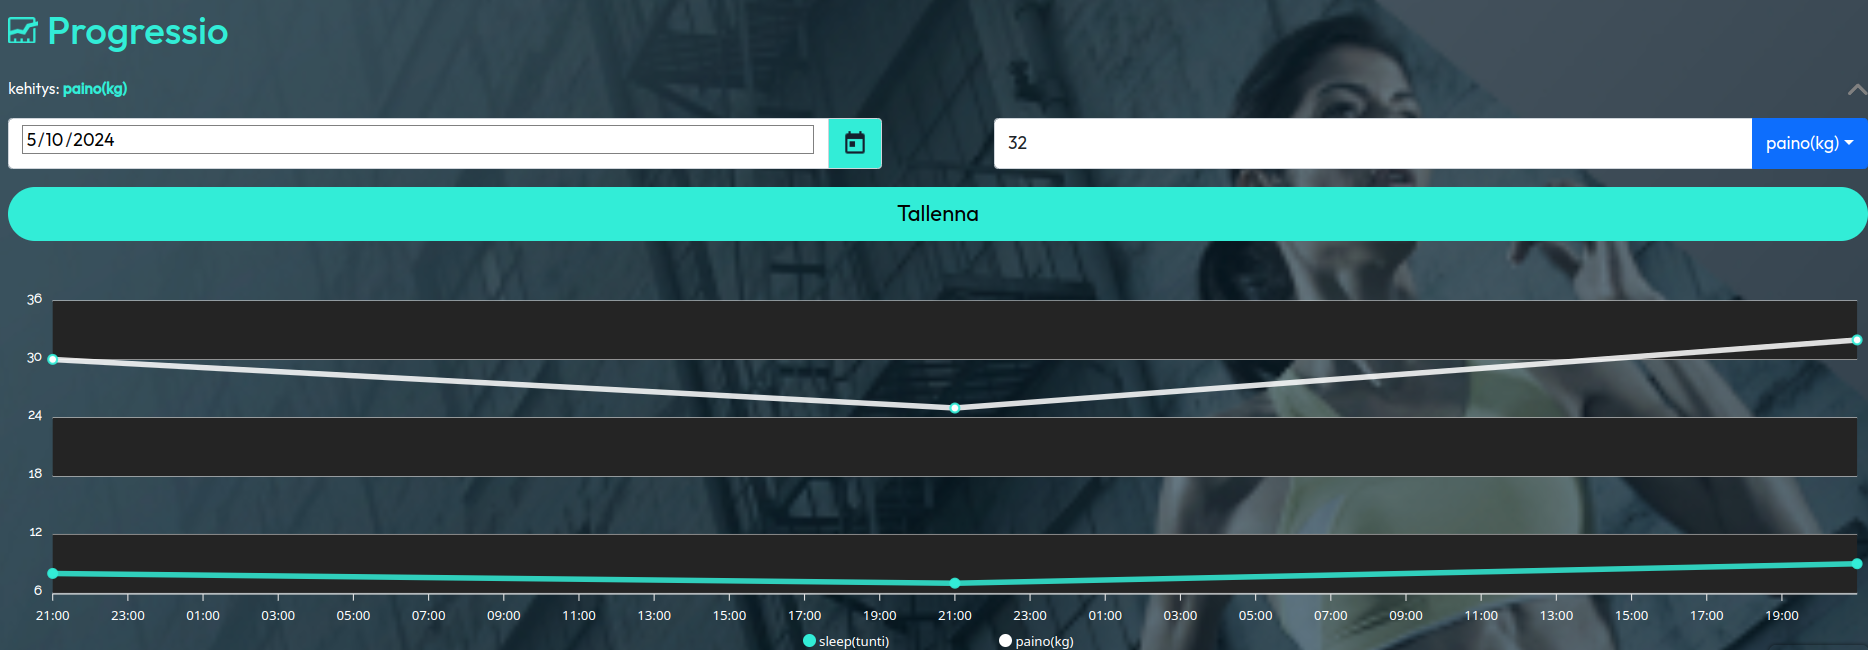
\includegraphics[width = 15cm]{src/public/progressmulti.png}\\
Kuva \getImgCount {}. Käyttäjän käyttöliittymä, muutoksien jälkeen 
\medskip

\bigskip
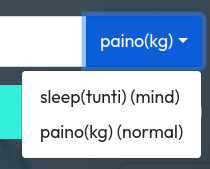
\includegraphics{src/public/progressselect.png}\\
Kuva \getImgCount {}. käyttöliittymän laskkuvalikosta
\medskip



Kuvassa \nextImageCount {} on päivitetty käyttäjän luomis- ja päivitys käyttöliittymä.
Käyttöliittymään on lisätty nappi, josta voi lisätä, nimetä ja poistaa mitattavia suureita käyttäjälle.
%selitä paremmin että voi uudelleen käyttää komponenttia. tarviin jonkun sanan tolle yhdistelmälle
Tekstikenttä ja poisto nappi on sisällytetty kuvan {\the\numexpr \theimgCounter + 2 } React komponenttiin "MeasurableThingElement". 
Tämä antaa mahdollisuuden lisätä uusia kenttiä, tekemällä uuden instanssin komponentista.
%

\bigskip
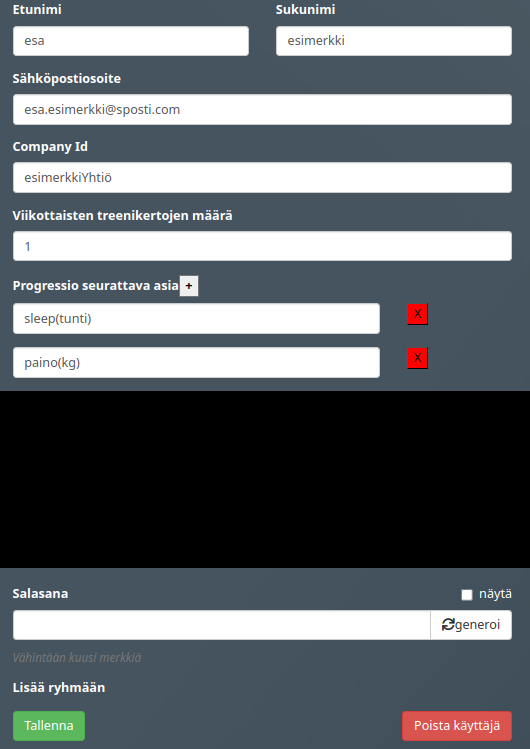
\includegraphics[width = 10cm]{src/public/oppar/adminUserProfilePostcencoredroles.png}\\
Kuva \getImgCount {}. Käyttäjien luomis käyttöliittymä 
\bigskip


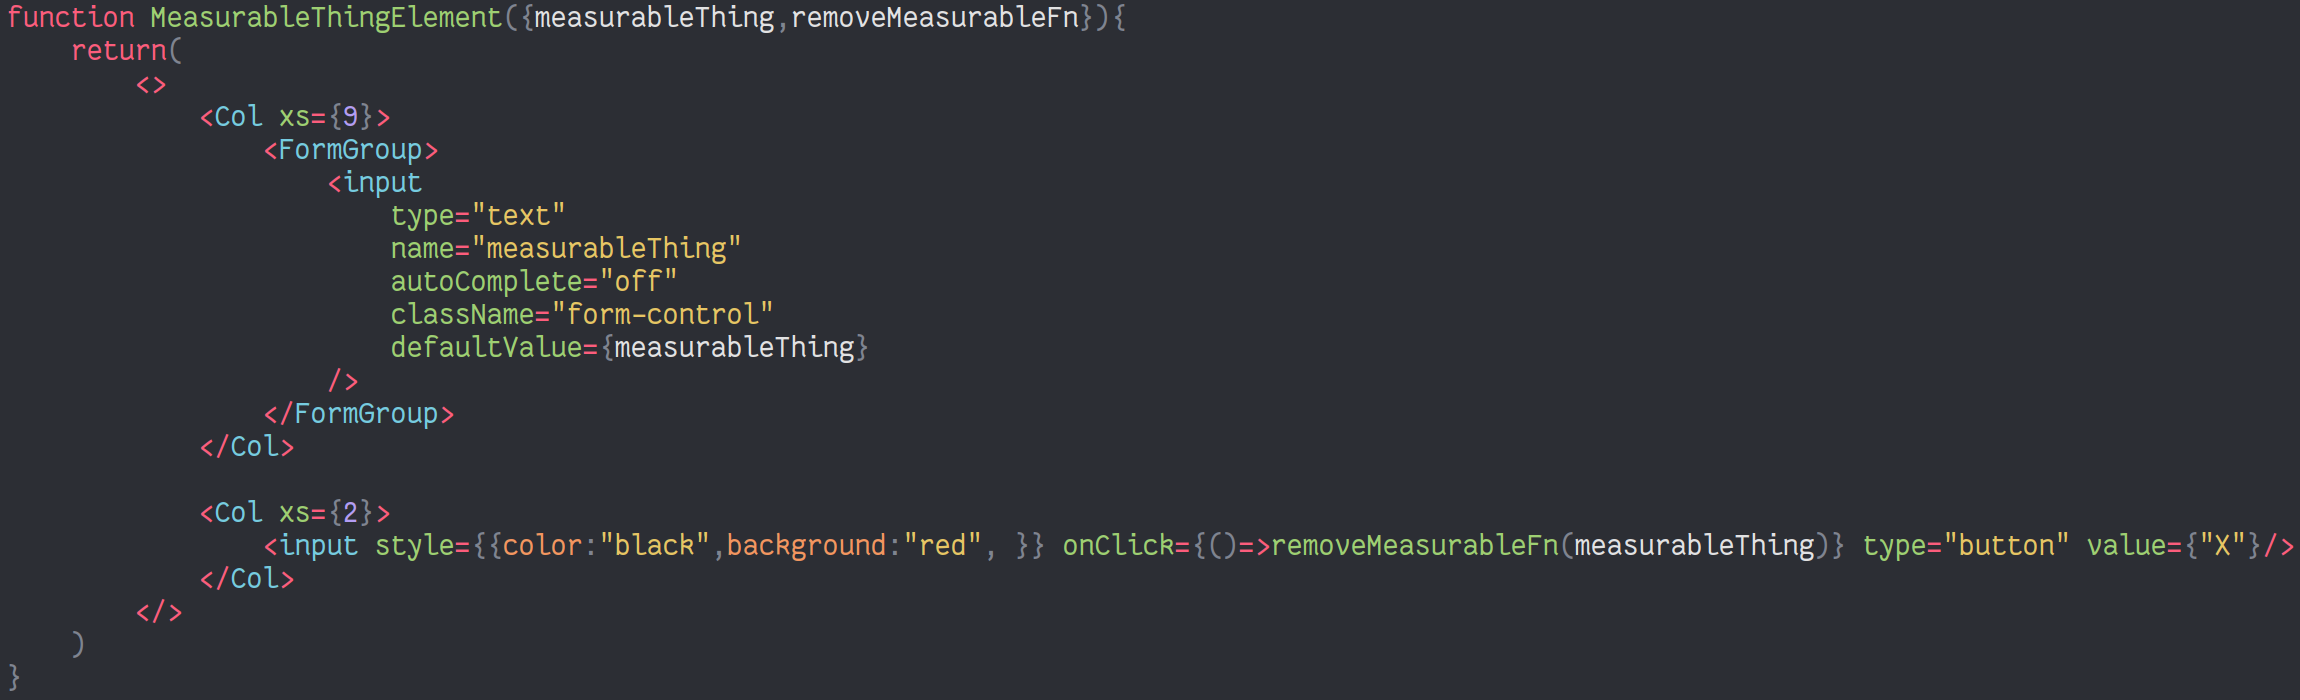
\includegraphics[width = 15cm]{src/public/oppar/measurableElementComponent.png}\\
Kuva \getImgCount {}. Mitattava elementti komponentti
\medskip

Komponentti on tilaton funktiokomponentti, johon annetaan mitattavan suurteen nimi ja poista funktio proppeina.
Poisto funktiota kutsutaan, kun painetaan punaista X nappia ja se poistaa mitattavan suurteen käyttäjän profiilista ja elementin käyttöliittymästä.
%{\the\numexpr \theimgCou:nter + 2 }
\medskip










\iffalse
% tämä on väärässä paikassa.  tai poistetaan kokonaan
Entisessä käyttöliittymässä kuvassa \nextImageCount {} on vain yksi teksti kenttä, josta pystyi muuttamaan measurableThing ominaisuuden nimeä.

%toinen paragraafi
\bigskip


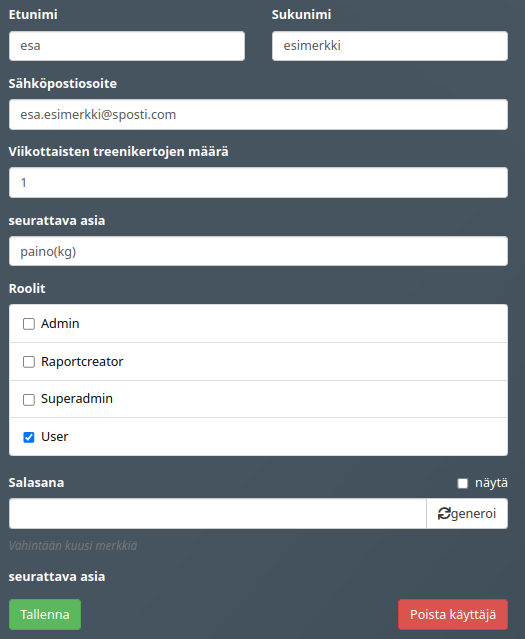
\includegraphics[width = 10cm]{src/public/oppar/adminUserProfilePre.png}\\
Kuva \getImgCount {}. Käyttäjän luomis käyttöliittymä ennen muutoksia (cencor roles?)
\medskip

\fi










